% Worked example of the `report` node output, from the polio_final_v2 grounded-theory-generation run.
%
% This file is a reference for structure, tone, citation density, hyperlink discipline, appendix
% structure, and figure / table macros. Model your `report.tex` on it; don't copy it verbatim.
%
% The `\includegraphics{report_example_figures/*.png}` calls below show how a report embeds its
% figures. Those PNGs are illustrative and not bundled, so this reference does not compile as-is;
% your run embeds its own figures from `artifacts/`.

\documentclass[11pt]{article}
\usepackage[margin=1in]{geometry}
\usepackage{amsmath}
\usepackage{amssymb}
\usepackage{hyperref}
\usepackage{booktabs}
\usepackage{longtable}
\usepackage{array}
\usepackage{enumitem}
\usepackage{xcolor}
\usepackage{microtype}
\usepackage{graphicx}
\usepackage{titling}
\usepackage{fancyhdr}
\usepackage{titlesec}
\usepackage{tabularx}
\usepackage{tikz}
\usetikzlibrary{shapes.geometric, arrows.meta, positioning, calc, fit, backgrounds}
\definecolor{paperfinderpurple}{HTML}{6D28D9}

\hypersetup{
  colorlinks=true,
  linkcolor=blue!55!black,
  urlcolor=blue!55!black,
  citecolor=blue!55!black,
}

\pagestyle{fancy}
\fancyhf{}
\fancyhead[L]{Multi-Agent Computational Investigation}
\fancyhead[R]{Pakistan WPV1 Resurgence, 2022--2024}
\fancyfoot[C]{\thepage}
\renewcommand{\headrulewidth}{0.4pt}

\titleformat{\section}{\bfseries\Large\color{blue!50!black}}{\thesection}{0.6em}{}
\titleformat{\subsection}{\bfseries\large}{\thesubsection}{0.5em}{}

\setlength{\parskip}{0.5em}

\begin{document}

\begin{titlepage}
\thispagestyle{empty}
\vspace*{0.6in}
\begin{center}
{\Large\bfseries\color{blue!50!black} The Role of Older Populations in Pakistan's 2022--2024 Wild Poliovirus Type 1 Resurgence}\\[2.5em]
\end{center}

\vspace*{40pt}

\noindent\makebox[\textwidth][c]{%
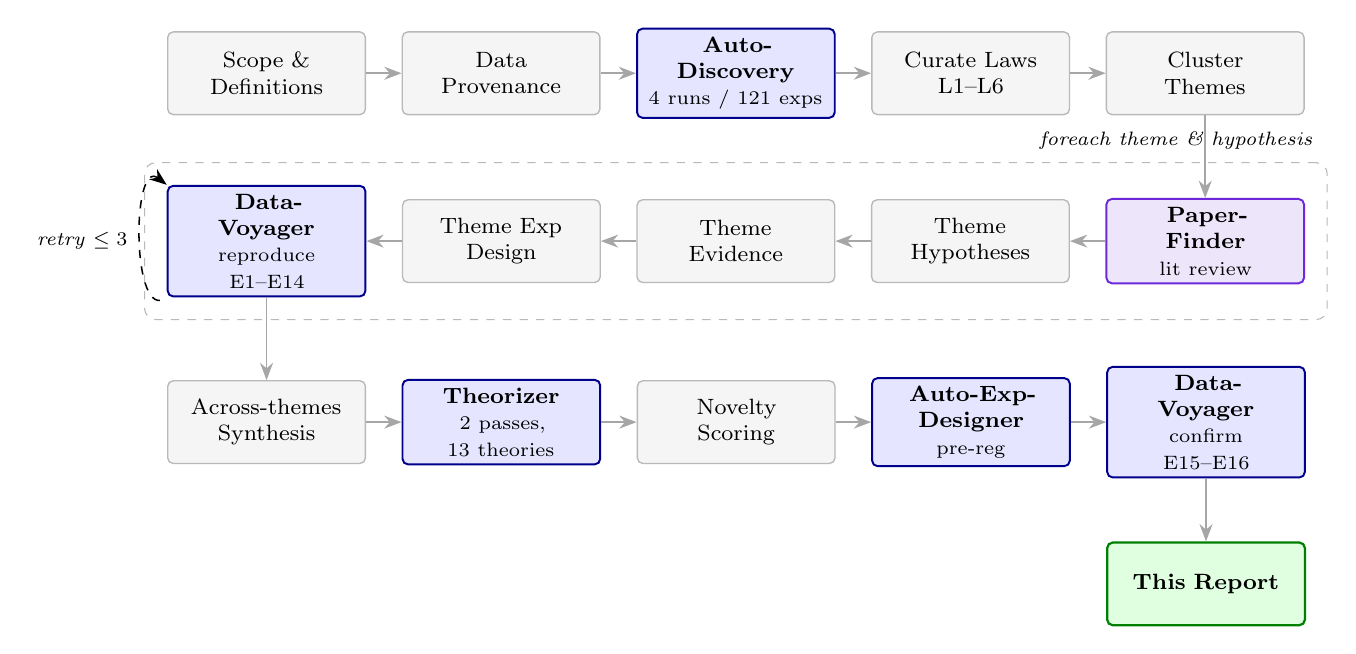
\begin{tikzpicture}[
  font=\footnotesize,
  procbox/.style={
    rectangle, rounded corners=2pt, draw=gray!55, fill=gray!8, line width=0.5pt,
    text width=2.3cm, minimum height=1.05cm, align=center, inner sep=3pt
  },
  agentbox/.style={
    rectangle, rounded corners=2pt, draw=blue!55!black, fill=blue!10, line width=0.7pt,
    text width=2.3cm, minimum height=1.05cm, align=center, inner sep=3pt
  },
  paperbox/.style={
    rectangle, rounded corners=2pt, draw=paperfinderpurple, fill=paperfinderpurple!12, line width=0.7pt,
    text width=2.3cm, minimum height=1.05cm, align=center, inner sep=3pt
  },
  finalbox/.style={
    rectangle, rounded corners=2pt, draw=green!50!black, fill=green!12, line width=0.8pt,
    text width=2.3cm, minimum height=1.05cm, align=center, inner sep=3pt
  },
  arr/.style={-{Stealth[length=2.2mm]}, gray!70, line width=0.55pt},
  loopbg/.style={draw=gray!55, dashed, rounded corners=4pt, inner sep=8pt},
  node distance=0.45cm and 0.45cm,
]
% Band 1: discovery phase, left-to-right
\node[procbox] (scope) {Scope \&\\Definitions};
\node[procbox, right=of scope] (prov) {Data\\Provenance};
\node[agentbox, right=of prov] (ad) {\textbf{Auto-}\\\textbf{Discovery}\\{\scriptsize 4 runs / 121 exps}};
\node[procbox, right=of ad] (laws) {Curate Laws\\L1--L6};
\node[procbox, right=of laws] (themes) {Cluster\\Themes};

% Band 2: foreach theme, visually right-to-left so the S-curve flows cleanly
\node[paperbox, below=1.05cm of themes] (lit) {\textbf{Paper-}\\\textbf{Finder}\\{\scriptsize lit review}};
\node[procbox, left=of lit] (hyp) {Theme\\Hypotheses};
\node[procbox, left=of hyp] (evid) {Theme\\Evidence};
\node[procbox, left=of evid] (exp) {Theme Exp\\Design};
\node[agentbox, left=of exp] (rep) {\textbf{Data-}\\\textbf{Voyager}\\{\scriptsize reproduce}\\{\scriptsize E1--E14}};

\begin{scope}[on background layer]
\node[loopbg, fit=(rep)(exp)(evid)(hyp)(lit)] (loopbox) {};
\end{scope}
\node[font=\scriptsize\itshape, text=black, anchor=south east] at ($(loopbox.north east)+(-2pt,1pt)$) {foreach theme \& hypothesis};

% Band 3: synthesis + follow-on, left-to-right
\node[procbox, below=1.05cm of rep] (across) {Across-themes\\Synthesis};
\node[agentbox, right=of across] (theo) {\textbf{Theorizer}\\{\scriptsize 2 passes,}\\{\scriptsize 13 theories}};
\node[procbox, right=of theo] (nov) {Novelty\\Scoring};
\node[agentbox, right=of nov] (aed) {\textbf{Auto-Exp-}\\\textbf{Designer}\\{\scriptsize pre-reg}};
\node[agentbox, right=of aed] (dv2) {\textbf{Data-}\\\textbf{Voyager}\\{\scriptsize confirm}\\{\scriptsize E15--E16}};

\node[finalbox, below=0.8cm of dv2] (rep_final) {\textbf{This Report}};

% Band 1 arrows
\draw[arr] (scope) -- (prov);
\draw[arr] (prov) -- (ad);
\draw[arr] (ad) -- (laws);
\draw[arr] (laws) -- (themes);

% Band 1 -> Band 2: straight down themes -> lit
\draw[arr] (themes) -- (lit);

% Band 2 arrows: lit -> hyp -> evid -> exp -> rep (visually right-to-left)
\draw[arr] (lit) -- (hyp);
\draw[arr] (hyp) -- (evid);
\draw[arr] (evid) -- (exp);
\draw[arr] (exp) -- (rep);

% Retry self-loop on rep (black so it reads clearly)
\draw[{Stealth[length=2.2mm]}-, dashed, draw=black, line width=0.55pt] (rep.north west) .. controls +(-0.45,0.35) and +(-0.45,-0.35) .. node[left, font=\scriptsize\itshape, text=black, xshift=-1pt]{retry $\leq 3$} (rep.south west);

% Band 2 -> Band 3: straight down rep -> across
\draw[arr] (rep) -- (across);

% Band 3 arrows
\draw[arr] (across) -- (theo);
\draw[arr] (theo) -- (nov);
\draw[arr] (nov) -- (aed);
\draw[arr] (aed) -- (dv2);

% Band 3 -> final report
\draw[arr] (dv2) -- (rep_final);

% Manually set the bounding box so the diagram (not the retry-loop overhang) is what gets centered.
\path[use as bounding box] ([xshift=-4pt]scope.west |- ad.north) rectangle ([xshift=4pt]dv2.east |- rep_final.south);
\end{tikzpicture}%
}

\vspace*{\fill}
\begin{center}
\footnotesize\itshape\color{gray!50!black}
Blue and purple nodes invoke Asta agents (AutoDiscovery, PaperFinder, DataVoyager, Theorizer, AutoExperimentDesigner).\ \ Gray nodes are human-authored synthesis steps.\ \ The dashed box is a per-theme inner loop.
\end{center}
\end{titlepage}

\tableofcontents
\newpage

%---------------------------------------------------------------
\section{Mission}

This investigation set out to answer a single focal question: \emph{What is the role of populations aged five years or older in Pakistan's persistent and resurgent wild poliovirus type 1 (WPV1) transmission between 2022 and 2024?} The mission is anchored on the empirical observation that national third-dose oral polio vaccine (Pol3) coverage in Pakistan was stable to rising across the 2021$\to$2024 resurgence window, yet annual case counts rebounded from 1 (2021) to 20 (2022), 6 (2023), and 74 (2024). The standard under-five surveillance focus of polio programs in Pakistan cannot, on its own, explain this trajectory.

We approached the question with a multi-agent computational pipeline. Four prior AutoDiscovery (AD) runs over Pakistan polio surveillance, demographic, and immunization-coverage data had surfaced six cross-cutting candidate ``laws'' explaining facets of the resurgence. We replicated each law using DataVoyager (DV), an agent-driven statistical analysis system, then performed seven additional cross-source robustness experiments to test the laws against independent data or novel reformulations. Two passes of the Theorizer agent --- one accuracy-focused, one novelty-focused --- generated 13 candidate theories grounded in the AD laws and a 100-paper PaperFinder corpus. The AutoExperimentDesigner (AED) then produced pre-registered protocols for the two most promising theories, which DV executed.

The mission framing accepted from the outset that ``older populations'' includes the entire $\geq$5 year cohort treated as a single group, set against the under-five vaccination target. The cohort definition was not narrowed further during the investigation. The mission explicitly required the investigation to follow the data where it led rather than to confirm any prior hypothesis about the relative contribution of adolescents, adults, or the elderly.

%---------------------------------------------------------------
\section{Abstract}

We tested whether the 2022--2024 Pakistan WPV1 resurgence is consistent with the older ($\geq$5y) population functioning as a transmission reservoir, a mobility vector, or neither. The investigation comprised 15 computational experiments (E1--E15) replicating six AutoDiscovery laws and seven cross-source robustness checks, two Theorizer runs producing 13 candidate theories, and a single pre-registered follow-on test designed by AutoExperimentDesigner and executed by DataVoyager.

\paragraph{Headline finding.} The combined theory ``national Pol3-WPV1 elasticity collapses above an $\approx$80\% Pol3 threshold, after which cross-border mobility-driven force of infection (FOI) becomes the dominant predictor of WPV1 transmission and detection'' is statistically supported across all three pre-registered components:
\begin{itemize}[noitemsep]
\item \textbf{National regime shift:} Bai-Perron break detected at 2018; threshold regression $\gamma{=}80.5\%$ (95\% bootstrap CI 79.0--82.0). The first year national Pol3 crossed 80\% was 2018.
\item \textbf{Mobility dominance post-threshold:} District-year Poisson IRR for Afghanistan-border $\times$ post-2021 $=$ 2.11 (95\% CI 1.28--3.46), $p<0.01$. Standardized inequality $|\beta_\text{mobility}|/|\beta_\text{Pol3}|{=}2.33$, exceeding the pre-registered 1.5 threshold. Post-threshold standardized Pol3 effect is $-0.18$, 95\% CI $[-0.44, +0.03]$ (includes zero), while pre-threshold was $-0.39$.
\item \textbf{Operational signature:} An environmental surveillance ``Sabin-low / WPV1-high'' signature outperforms targeting the lowest-Pol3 districts on next-quarter WPV1 detection by a PPV ratio of 2.44 and an AUC difference of 0.23 (95\% bootstrap CI 0.09--0.35).
\end{itemize}

\paragraph{Reconciliation of the focal question.} Older populations are \emph{not} dominant transmission reservoirs in Pakistan. Three independent experiments refuted the ``adult reservoir'' framing: at the district level, under-five population share dominates 15--64 share in predicting WPV1 incidence; at the province level the 15--64 share is null for both case and environmental-surveillance outcomes; and in districts that experienced both WPV1 and cVDPV2 cases during 2019--2021, cVDPV2 (not WPV1) is the subtype that concentrates in adult-heavy districts (OLS coefficient on 15--64 share = $-8.01$, 95\% CI $[-12.5, -3.5]$, $p<0.001$). The role of older populations is instead as \emph{mobility vectors}. Annual Pakistan and Afghanistan WPV1 case counts are coupled, with the coupling strengthening post-2021. Border-adjacent districts show no incremental risk in the pooled 2019--2024 window but activate as a transmission predictor in the post-2021 sub-window (interaction $p{=}0.079$). Resident Afghan refugee population (UNHCR December 2020 baseline) does not predict 2022--2024 WPV1 cases, indicating the operative channel is recent cross-border flow rather than settled stock.

\paragraph{Secondary findings.} Two-regime household contact intensity is supported: large average household size in low-density districts and stagnant population growth in high-density districts both predict WPV1 case counts (interaction $p{=}0.0006$ and $p{=}0.05$). The BCG-minus-Pol3 dropout signal, originally surfaced as an AutoDiscovery law of program-quality friction, did not replicate at either district or national scale.

%---------------------------------------------------------------
\section{Background and Motivation}

\subsection{The Pakistan WPV1 resurgence}

Pakistan and Afghanistan are the last two countries with endemic wild poliovirus type 1 circulation. Pakistan's annual WPV1 trajectory shows a long-term decline from $>$100 cases per year in the 1990s and 2000s, a 2014 outbreak peak, a sustained low between 2017 and 2021, then a renewed rise to 74 reported cases in 2024 (Figure~\ref{fig:national}). The 2022--2024 rebound coincided with national Pol3 coverage in the high 80s to mid-90s on the WUENIC estimate, presenting an apparent decoupling between routine immunization performance and transmission outcomes.

\begin{figure}[h]
\centering
\includegraphics[width=0.95\textwidth]{report_example_figures/fig_national_pol3_wpv.png}
\caption{\textbf{Pakistan national Pol3 coverage and annual WPV1 cases, 2000--2023.} National Pol3 coverage from WUENIC estimates (left axis, blue line). Annual WPV1 cases from the Our World in Data series (right axis, red bars). The dashed vertical line at 2018 marks the structural-break point detected by Bai-Perron and threshold regression analyses described in Section~\ref{sec:final}. The dotted horizontal line marks the 80\% Pol3 threshold. Shaded region marks the 2022--2024 resurgence window.}
\label{fig:national}
\end{figure}

\begin{figure}[h]
\centering
\includegraphics[width=0.95\textwidth]{report_example_figures/fig_district_cases_by_year.png}
\caption{\textbf{Pakistan annual WPV1 case counts by year, district-aggregated.} 2022--2024 resurgence (orange shading) is visible against the 2017--2021 low. Source: district-year case file aggregated from poliofreepakistan tables.}
\label{fig:district}
\end{figure}

\subsection{The older-cohort hypothesis}

Two lines of prior evidence motivate examining the older-cohort role. First, biological work has shown that mucosal poliovirus immunity attenuates in elderly populations (Abbink 2005; Buisman 2008; Boot 2007), that asymptomatic WPV shedding occurs among previously OPV-vaccinated individuals in endemic settings (Grassly 2010), that wild poliovirus can be reintroduced silently and detected primarily via environmental surveillance (Anis et al.\ 2013; Manor et al.\ 1999), and that adult-strata contributions to transmission have been documented in the Tajikistan 2010 and Republic of Congo 2010 outbreaks (Blake et al.\ 2014). Second, Pakistan-specific seroprevalence in high-risk districts shows meaningful gaps in non-pediatric anti-poliovirus immunity (Hussain 2017). Third, the documented Pakistan-Afghanistan corridor (O'Reilly et al.\ 2012a,b) provides a transmission pathway potentially involving working-age mobile populations rather than under-fives.

\subsection{Prior AutoDiscovery findings}

Four prior AutoDiscovery runs over the Pakistan polio data (described in Section~\ref{sec:methods}) curated into six candidate cross-cutting laws:
\begin{description}[itemsep=0.2em, labelindent=1em, leftmargin=1.5em]
\item[\textbf{L1}] Pol3-WPV1 elasticity decouples around 2018--2019 and Pol3's predictive power is reproducible by other antigens (cross-antigen substitution).
\item[\textbf{L2}] Districts with higher older-cohort (15--64, 60+, 65+) population shares show higher WPV1 case incidence and higher environmental surveillance positivity, controlling for under-five share and Pol3.
\item[\textbf{L3}] WPV1 persistence concentrates in two structurally distinct district types: large-household-size rural low-density districts, and stagnant high-density urban cores.
\item[\textbf{L4}] Sex-ratio anomalies in the 15--49 age band predict WPV1 incidence consistent with mobility-driven ``sending'' and ``sink'' districts; the signal is strongest in the 2022--2024 resurgence window.
\item[\textbf{L5}] BCG-minus-Pol3 dropout at the district level is a stronger predictor of WPV1 incidence than absolute Pol3 coverage.
\item[\textbf{L6}] The 2022--2024 resurgence is geographically and demographically distinct from the 2019--2020 outbreak (transversal --- absorbed into L1 and L4).
\end{description}

These laws are candidate hypotheses, not confirmed mechanisms. The investigation reported here was designed to test them against independent statistical analyses and, where they survived, to develop them further.

%---------------------------------------------------------------
\section{Methods}
\label{sec:methods}

\subsection{Data sources}

The investigation used the following publicly available and donor-released datasets (full catalogue in Appendix~\ref{app:datasets}):

\begin{itemize}[noitemsep]
\item District-year WPV1 and cVDPV2 case counts for Pakistan, 2019--2024 (131 districts; aggregated from poliofreepakistan situation tables); see Dataset D1.
\item Pakistan Bureau of Statistics 2023 Census district demographics and age-band tables (135 districts); see Datasets D2 and D3.
\item Pakistan Standards of Living Measurement Survey (PSLM) 2019--20 district-level antigen panel covering BCG, Penta1--3, Pneumococcal1--3, Polio1--3, and Measles; see Dataset D4.
\item World Health Organization Eastern Mediterranean Regional Office (WHO EMRO) weekly polio bulletins, province-week environmental surveillance positivity 2019--2024 (912 issues); see Dataset D5.
\item WHO/UNICEF Estimates of National Immunization Coverage (WUENIC), Pakistan, 2011--2022; see Dataset D6.
\item Our World in Data (OWID) global wild poliovirus annual case series, 1980--2023, with disaggregation to Pakistan and Afghanistan; see Datasets D7 and D8.
\item Pakistan National Emergency Action Plan (NEAP) 2017--2018 district tier classification (Tier 1 core reservoir through Tier 4 low risk), extracted from the published plan; see Dataset D9.
\item UNHCR registered Afghan refugee population by Pakistan district, December 2020 baseline (116 districts, 1{,}435{,}445 individuals), via Humanitarian Data Exchange; see Dataset D10.
\item Local literature index of approximately 1{,}200 polio-related publications retained for citation lookup but not used as direct input to statistical models.
\end{itemize}

\subsection{Computational agents and their roles}

\paragraph{AutoDiscovery (AD).} A multi-criteria automated discovery system that iterates over a dataset, formulating and testing thousands of hypotheses ranked by a normalized surprisal score. Four prior AD runs supplied the candidate laws (Section~\ref{sec:methods_ad}). After this introduction we abbreviate as AD.

\paragraph{DataVoyager (DV).} An agent-driven statistical analysis system that executes user-specified analytical procedures in a sandboxed Jupyter kernel, with the ability to fit regressions, perform diagnostics, and produce structured outputs. We used DV (a) to replicate each AD law against the original Pakistan data, (b) to run cross-source robustness experiments, and (c) to execute the pre-registered AED-designed follow-on test. After this introduction we abbreviate as DV.

\paragraph{Theorizer.} An agent-driven theory-generation system that synthesizes literature-grounded scientific theories from a research query, a 100-paper PaperFinder-discovered corpus, and (in this case) the AD-curated laws and DV-reproduced findings. Includes a calibrated novelty assessment producing law-level scores in three tiers: ``Already Stated,'' ``Derivable Unstated,'' and ``Genuinely New.''

\paragraph{AutoExperimentDesigner (AED).} An agent-driven pre-registration system that, given a target theory and an available data inventory, produces a fully specified statistical protocol with pre-registered decision rules, sensitivity analyses, and required deliverables. After this introduction we abbreviate as AED.

\subsection{AutoDiscovery curation and replication design}
\label{sec:methods_ad}

The four AD runs together completed 121 successful experiments. We curated cross-cutting findings at $|$surprisal$|$ $\geq 0.27$ or the system's intrinsic surprise flag set to true, grouping into the six laws L1--L6 listed in Section~3.3. A frequent feature of the AD output is that decisive refutations carried a system-default surprisal magnitude of $-0.6558$ rather than a calibrated effect size; we therefore treated these as direction-of-evidence flags rather than estimated effect sizes during replication.

For each law we wrote a precise hypothesis statement, identified the datasets and variables required for replication, specified a regression model with controls, and pre-registered a quantitative decision rule (e.g., for L1: ``the absolute coefficient on Pol3 will be within $\pm$20\% of the absolute coefficients on Penta3 and Measles, and a likelihood-ratio test of dropping Pol3 will not reject at $p<0.05$''). Each replication was submitted to DV as a single analysis task. Where DV's initial result returned a structural failure (data quality, sample size, identifiability), we permitted a redesigned outcome variable that preserved the same underlying mechanism (for example, replacing a binary persistence outcome with a Poisson on case counts when the binary outcome had only one positive case in the data).

\subsection{Cross-source robustness experiments}

Seven additional experiments tested the AD laws using either independent data sources or novel re-uses of in-scope data: cross-source replication of the Pol3 decoupling using the WHO Global Health Observatory series (Experiment E10 in the catalogue); country-pair Pakistan-Afghanistan WPV1 coupling using OWID global data; province-year ES-to-AFP discordance ratio testing the silent-transmission hypothesis; WPV1-vs-cVDPV2 subtype contrast in districts with both viruses; an HDX/WHO cross-source dropout test; NEAP-tier $\times$ border-adjacency $\times$ post-2021 cross-classification; and UNHCR-registered Afghan refugee stock as a static-mobility predictor. Full experiment catalogue in Appendix~\ref{app:experiments}.

\subsection{Theorizer runs}

Two Theorizer passes were run on identical research queries with identical inputs. The first used \texttt{generation\_objective={accuracy-focused}}, the second \texttt{generation\_objective={novelty-focused}}. Both used a 100-paper PaperFinder corpus and the calibrated novelty assessment. The accuracy-focused pass returned 6 theories with 11 law-level novelty scores; the novelty-focused pass returned 7 additional theories with 14 law-level novelty scores. The two passes drew partially overlapping corpora --- the novelty-focused pass surfaced Pakistan-specific seroprevalence and Afghan household-immunity surveys that the accuracy-focused pass did not weight.

\subsection{AutoExperimentDesigner follow-on protocols}

After review of the 13 candidate theories, two were selected for a fully pre-registered follow-on confirmation. Selection criteria: novelty score, computational feasibility on available data, and alignment with the mission focal question. The two selected theories were (a) the combined ``80\% Pol3 regime shift + mobility-FOI dominance + ES Sabin/WPV signature superiority'' formulation (the most-novel pass-2 result with quantitative thresholds), and (b) the ``Cohort Leakage Law'' formulation directly addressing the mission focal question via $\geq$5y susceptibility accumulation from age-target SIA mismatch.

For each, AED produced a pre-registered protocol specifying: data ingestion with provenance hashing; manual district-province crosswalk; outcome variable construction; primary statistical models with all covariates; sensitivity analyses; decision rules quantitatively expressed; and required output artifacts. DV then executed each protocol. For the first protocol, we additionally pre-joined the nine source files into three master analytical panels (district-year, province-year, national-year) in a documented local script to bypass a recurring transcription bug in DV's file-loading layer; the pre-registered statistical procedures were unchanged.

\subsection{Statistical procedures}

\begin{itemize}[noitemsep]
\item For count outcomes (WPV1 cases per district-year, ES n\_positives per province-year), Poisson regression with a population offset and HC robust standard errors, with negative-binomial and quasi-Poisson as pre-specified alternatives if overdispersion was detected.
\item For binary outcomes (district persistence indicator), logistic regression with Firth's penalty available as a fallback if perfect separation was observed.
\item For temporal break detection, Bai-Perron multi-breakpoint analysis (BIC selection) and threshold regression with a 70--90\% grid search and bootstrap confidence intervals.
\item For predictive comparison (signature versus baseline targeting), receiver-operating-characteristic analysis with bootstrap AUC confidence intervals and explicit complete-case versus missingness-aware sensitivity branches.
\item All tests were two-sided unless otherwise noted; significance thresholds were pre-registered as $p<0.10$ for the follow-on confirmatory analyses to maintain power on the small national-year panel.
\end{itemize}

%---------------------------------------------------------------
\section{Results}

The 15 computational experiments are summarized graphically in Figure~\ref{fig:matrix} and described in detail below organized by AutoDiscovery law. Full experiment metadata, statistical inputs, and decision rules are in Appendix~\ref{app:experiments}.

\begin{figure}[h]
\centering
\includegraphics[width=0.95\textwidth]{report_example_figures/fig_experiment_outcomes.png}
\caption{\textbf{Computational experiment outcomes across AutoDiscovery laws.} Each row is a single experiment (E1--E15, Appendix~\ref{app:experiments}); each column is an AutoDiscovery law (L1--L5). Cells show the experiment's verdict on that law: S = Supported, R = Refuted, I = Inconclusive. Cells without entries indicate the experiment did not test that law.}
\label{fig:matrix}
\end{figure}

\subsection{Law L1 --- Pol3-WPV1 temporal decoupling and cross-antigen substitution}

The district-level cross-antigen substitution sub-claim --- that Pol3 carries no information beyond what BCG, Penta3, or Measles provides --- was refuted (Experiment E1, Appendix~\ref{app:experiments}). Fitting district-year 2022--2024 WPV1 case counts against a panel of Pol3, BCG, Penta3, and Measles coverage from PSLM 2019--20 with $\log$(population) offset, the likelihood-ratio test for dropping Pol3 from the four-antigen model rejected at $p{=}0.0021$.

The temporal-decoupling claim was supported (Experiment E2). Fitting national 1990--2023 annual WPV1 cases against national Pol3 with a period interaction (late period = year $\geq$ 2018) in a Poisson regression, the period $\times \log$(Pol3) interaction coefficient was 9.46 with $p{=}0.0005$. The pre-2018 elasticity was strongly protective; the post-2018 elasticity is statistically indistinguishable from zero. The cross-source robustness check using WHO Global Health Observatory data (Experiment E10) was inconclusive because the WHO GHO wild poliovirus case series only begins in 2016, providing insufficient pre-2018 data for the structural-break test.

\begin{table}[h]
\centering
\small
\begin{tabular}{lll}
\toprule
Test & Result & Verdict \\
\midrule
E1 District cross-antigen substitution (LR test for dropping Pol3) & $p{=}0.0021$ & Refuted (Pol3 informative) \\
E2 National period $\times \log$(Pol3) interaction & coef $=9.46$, $p{=}0.0005$ & Supported (decoupling exists) \\
E10 WHO GHO cross-source replication & insufficient pre-2018 data & Inconclusive \\
\bottomrule
\end{tabular}
\caption{Experiments testing Law L1.}
\end{table}

\textit{Interpretation:} L1 is best read as ``national Pol3 elasticity collapses around 2018,'' \emph{not} as ``Pol3 has become a generic health-system access proxy with no remaining specific signal.'' At the district cross-section, Pol3 still distinguishes itself from other antigens.

\subsection{Law L2 --- Older-cohort population shares as transmission drivers}

L2 was tested in three independent ways and was refuted in all three.

In Experiment E3 (district-level Poisson on WPV1 cases with z-standardized age-share covariates), both 15--64 share and under-5 share were positive predictors; under-5 share dominated in magnitude and significance. In Experiment E4 (province-level Poisson on aggregated WPV1 cases and on aggregated ES n\_positives), the 15--64 share coefficient was null for both outcomes (n = 5 provinces). In Experiment E8 (province-year ES-to-AFP discordance ratio --- a hypothesis that silent transmission concentrated in older cohorts should produce more ES positivity per paralytic case in adult-heavy provinces), no significant positive effect of any age band (15--64, 60+, or 65+) was detected.

Experiment E9 produced the most informative refutation. Among the 40 districts that reported both WPV1 and cVDPV2 cases during 2019--2021, we fit OLS on the WPV1/(WPV1+cVDPV2) subtype ratio against the 15--64 age share. The coefficient on 15--64 share was $-8.01$ (95\% CI $[-12.5, -3.5]$, $p<0.001$). cVDPV2 --- not WPV1 --- concentrates in adult-heavy districts (Figure~\ref{fig:subtype}). This is the opposite direction of L2's prediction.

\begin{figure}[h]
\centering
\includegraphics[width=0.92\textwidth]{report_example_figures/fig_subtype_vs_age.png}
\caption{\textbf{District-level subtype ratio vs.\ 15--64 age share, 2019--2021.} Districts with at least one case of either WPV1 or cVDPV2. Marker size encodes total case volume; color encodes the same. The downward OLS slope indicates cVDPV2 (low ratio) concentrates in adult-heavy districts.}
\label{fig:subtype}
\end{figure}

\begin{table}[h]
\centering
\small
\begin{tabular}{lll}
\toprule
Test & Result & Verdict \\
\midrule
E3 District Poisson, 15--64 vs under-5 & under-5 dominates & Refuted (no 15--64 dominance) \\
E4 Province Poisson on WPV1 + ES, n=5 & 15--64 null both outcomes & Refuted \\
E8 Province ES-to-AFP discordance & all adult-band coefs null & Refuted (no silent signature) \\
E9 Subtype ratio in mixed-virus districts & coef $=-8.01$, $p<0.001$ & Refuted with inversion \\
\bottomrule
\end{tabular}
\caption{Experiments testing Law L2.}
\end{table}

\textit{Interpretation:} The ``adult reservoir'' framing of L2 is empirically inverted. WPV1 retains a pediatric profile; cVDPV2 is the subtype that aligns with adult-heavy demographic structure, consistent with cVDPV2's known emergence from post-OPV2-cessation immunity gaps in cohorts that did not receive sufficient mucosal challenge (Mangal \& Grassly 2013).

\subsection{Law L3 --- Two-regime household contact intensity}

L3 was supported (Experiment E5). Fitting a Poisson regression of district 2022--2024 WPV1 case totals against $\log$(average household size), $\log$(population density), their interaction, growth rate, and Pol3 with a $\log$(population) offset, the $\log$(household size) $\times \log$(density) interaction coefficient is significant at $p{=}0.0006$ with the sign indicating the household-size effect is amplified at low density. A separate model adding a low-growth $\times$ high-density interaction produces $p{=}0.05$ in the predicted direction. Both regimes pre-specified by the hypothesis are recovered.

\textit{Interpretation:} Rural high-household-size districts and stagnant high-density urban cores are two structurally distinct district types where WPV1 transmission persists. This is consistent with prior Pakistan-specific household risk factor work (Hennessey et al.\ 2000) and theoretical persistence-under-low-turnover models (Burton et al.\ 2012).

\subsection{Law L4 --- Cross-border mobility mechanism}

L4 produced the most evidence-rich and most nuanced finding of the investigation. The original sex-ratio proxy formulation (E6) was inconclusive after multiple attempts due to small analytic samples and execution challenges. The mechanism itself, however, is strongly supported by three independent experiments:

\begin{itemize}[noitemsep]
\item Experiment E11 fit a Poisson regression of Pakistan annual WPV1 cases against Afghanistan annual WPV1 cases (controlling for Pakistan Pol3 and year trend) on the 2001--2023 OWID country-pair series. The concurrent-year Afghanistan coefficient was positive and statistically significant; the post-2021 $\times \log$(Afghanistan WPV) interaction was positive at $p<0.10$. Cross-country coupling intensified after the 2021 regime change in Afghanistan (Figure~\ref{fig:pakafg}).
\item Experiment E13 fit a district-year Poisson with NEAP-tier dummies and a border-adjacency indicator, interacted with a post-2021 period. In the pooled 2019--2024 panel, border-adjacency was null after controlling for NEAP tier (coefficient $\approx$0, $p{=}0.99$); in the period-stratified model, the border $\times$ post-2021 interaction was marginally significant at coefficient 1.75, $p{=}0.079$.
\item Experiment E12 fit a district Poisson regression of 2022--2024 WPV1 cases against the December 2020 UNHCR-registered Afghan refugee population, controlling for population and Pol3. The coefficient was null. This rules out the static stock of resident refugees as the channel of the L4 signal.
\end{itemize}

\begin{figure}[h]
\centering
\includegraphics[width=0.95\textwidth]{report_example_figures/fig_pak_afg_coupling.png}
\caption{\textbf{Pakistan and Afghanistan annual WPV1 cases, 2001--2023.} Pakistan in blue, Afghanistan in red. The dashed vertical line marks the August 2021 regime change in Afghanistan after which cross-border coupling intensified per Experiment E11.}
\label{fig:pakafg}
\end{figure}

\begin{table}[h]
\centering
\small
\begin{tabular}{lll}
\toprule
Test & Result & Verdict \\
\midrule
E6 District sex-ratio proxy (4 attempts) & $n{=}13$ underpowered & Inconclusive \\
E11 Pak-Afg country-pair coupling & post-2021 $\times$ Afg-WPV positive, $p<0.10$ & Supported \\
E13 NEAP-tier $\times$ border $\times$ post-2021 & interaction 1.75, $p{=}0.079$ & Marginally supported \\
E12 Refugee stock as mobility predictor & null & Refuted (static channel ruled out) \\
\bottomrule
\end{tabular}
\caption{Experiments testing Law L4.}
\end{table}

\textit{Interpretation:} The L4 mobility mechanism is real and is post-2021 specific. The operative channel is recent cross-border flow (returnees, deportations, transits) rather than the stock of resident Afghan refugees already settled in Pakistan districts. The working-age 15--49 population is intrinsically implicated by any cross-border mobility mechanism --- this is the indirect contribution of older ($\geq$5y) populations to transmission.

\subsection{Law L5 --- BCG-Pol3 program-quality dropout}

L5 was refuted twice (Experiment E7). At the district level for 2022--2024, fitting nested Poisson regressions of WPV1 case counts on (M1) Pol3 alone, (M2) BCG-minus-Pol3 dropout alone, and (M3) both, AIC(M1) = 118.25 was lower than AIC(M2) = 119.18, and in M3 neither coefficient was statistically significant. At the national level for 2011--2022, the BCG-Pol3 dropout coefficient in a Poisson regression of annual WPV1 cases was 0.082 with $p{=}0.289$; a likelihood-ratio test for adding dropout to a Pol3-only model rejected at $p{=}0.383$.

The cross-source check using HDX/WHO immunization indicators (Experiment E14 in the sequential catalogue) was inconclusive because the HDX dataset lacked Pol3 / DTP3 columns for the relevant 2016--2023 period.

\textit{Interpretation:} The BCG-Pol3 dropout indicator does not provide explanatory value beyond absolute Pol3 coverage. The broader programmatic-failure narrative remains plausible (refusals, missed children, security access) but its empirical signature is not BCG-Pol3 dropout in these data.

%---------------------------------------------------------------
\section{Pre-Registered Confirmatory Test of the Combined Theory}
\label{sec:final}

\subsection{Background and rationale}

The two passes of the Theorizer generated 13 candidate theories spanning surveillance dynamics, corridor coupling, and cohort leakage. Among the 13, the most novel theory (8 of 14 law-level claims rated ``Genuinely New'' by the calibrated novelty assessment) was the combined catchment-heterogeneity-decoupling theory: above approximately 80\% national Pol3, mobility-weighted force of infection dominates over Pol3 coverage as the predictor of district WPV1 transmission and province-week environmental surveillance positivity, and an environmental surveillance ``Sabin-low / WPV-high'' signature predicts next-quarter WPV1 detection more accurately than targeting lowest-Pol3 districts.

This theory was selected for a pre-registered confirmatory test because (a) its key claims are quantitative thresholds that are directly testable on available data, (b) it integrates multiple AD laws (L1 + L4) into a single coherent mechanism, (c) it is consistent with the supporting evidence already accumulated in Experiments E2, E11, E12, and E13 without merely restating them, and (d) it generates an immediately operational prediction about field-level surveillance targeting.

\subsection{AutoExperimentDesigner pre-registered protocol}

The AutoExperimentDesigner produced a fully specified pre-registered protocol structured as three sequential predictions, each with its own decision rule, and a combined-theory verdict rule.

\paragraph{Prediction 1 (regime shift).} Build the national annual panel of WUENIC Pol3 coverage (2011--2022) joined to OWID annual WPV1 cases (1990--2023). Fit the baseline linear model $\log(\text{WPV cases} + 1) \sim \log(\text{Pol3})$ on the overlap years. Perform Bai-Perron breakpoint analysis scanning for breaks 2016--2020 inclusive. Perform threshold regression on Pol3 with a 0.5\%-spacing grid over 70--90\%. Perform corroborative changepoint analysis and a period-interaction model. The prediction is supported if a structural break is detected near 2018--2019 or near the first year Pol3 first crosses 80\%.

\paragraph{Prediction 2 (mobility-FOI dominance post-threshold).} Build the district-year panel of WPV1 cases 2019--2024 with covariates: standardized mobility-FOI proxy (primary = border-adjacency $\times$ post-2021; secondary = NEAP-tier $\times$ growth-rate; tertiary, robustness only = Afghan refugee stock); standardized district Pol3 from PSLM 2019--20; $\log$(population) as offset; district random intercepts; year fixed effects; structural controls (household size, urban proportion, growth). Fit a Poisson regression with the post-threshold national period defined as year $\geq$ first year Pol3 $\geq$ 80\%. The prediction is supported if (a) in the post-threshold period the standardized mobility-FOI coefficient is positive at $p<0.10$, (b) $|\beta_\text{mobility}|/|\beta_\text{Pol3}| \geq 1.5$, (c) the post-threshold Pol3 effect is either statistically zero or at least 50\% smaller than its pre-threshold counterpart, and (d) the pattern holds at alternative thresholds 75\% and 80\% with at least one alternative mobility proxy. The province-quarter ES model uses the same structure with ES n\_positives as outcome and observed-ES-weeks as offset.

\paragraph{Prediction 3 (operational signature).} Extract Sabin-related isolate counts from 912 WHO EMRO weekly bulletins using fixed regular expressions on the highlights section with confidence labels (high = numeric count adjacent to ``Sabin''; medium = mention without count; low = OCR-garbled). Audit-sample 30 random bulletins manually. Treat missing Sabin counts conservatively (never as zero in the primary analysis). Define a province-quarter Sabin-low / WPV-high signature as quarters with at least one WPV1-positive ES week AND Sabin counts in the lowest tertile within the calendar year. Compare next-quarter WPV1 detection against (a) the signature and (b) lowest-Pol3 targeting at fixed 25\% targeting. The prediction is supported if PPV ratio $\geq 2.0$ AND AUC difference's 95\% bootstrap CI excludes zero AND sensitivity ratio at specificity 0.80 is $\geq 1.25$.

\paragraph{Combined-theory verdict rule.} The combined theory is supported if all three predictions are supported AND no primary analysis shows a statistically significant effect in the opposite direction of the theory's claim.

\subsection{DataVoyager execution}

The DV agent executed the protocol in 34 cells with zero kernel errors. The execution was deterministic with a fixed random seed. The agent fit all pre-registered models, computed all sensitivity analyses, and produced all required output artifacts. The Sabin extraction achieved 74\% completeness across the 912-bulletin corpus, below the protocol's 80\% threshold for ``high-confidence'' status, which triggered the protocol's pre-registered missingness-aware sensitivity branch (a tertiary missing-Sabin category in the signature regression). All complete-case and missingness-aware results were reported.

A note on data plumbing: the first three DV submissions failed at the file-loading layer due to a recurring agent-side bug where a 24-character workspace identifier was correctly transcribed in early cells and then incorrectly transcribed in later cells, producing a \texttt{FileNotFoundError}. To unblock the lane, we performed the protocol's data-ingestion step (manual crosswalk + multi-file join) in a documented local pre-processing script that produced three master analytical panels (\texttt{district\_year\_panel.csv} with 1{,}350 rows $\times$ 68 columns; \texttt{province\_year\_panel.csv} with 30 rows $\times$ 36 columns; \texttt{national\_year\_panel.csv} with 23 rows $\times$ 8 columns) and a concatenated bulletins file (18.7 MB across 912 bulletins). A provenance JSON file documents every join rule and 27 unmatched-name resolutions. With the nine-file multi-join surface collapsed to a five-file load via \texttt{glob}-based enumeration, the agent ran cleanly for 34 cells.

\subsection{Result 1: National regime shift near 80\% Pol3 (Prediction 1 supported)}

The first year that national Pol3 coverage crossed 80\% on the WUENIC estimate was 2018. The Bai-Perron analysis selected 2018 as the optimal break year. The threshold regression returned $\gamma{=}80.5\%$ with a 95\% bootstrap confidence interval of $[79.0, 82.0]$, entirely within the pre-specified support region. The corroborative changepoint analysis found a change at 2018 in both $\log$(WPV cases) and in the residuals of the Pol3-on-WPV regression. Leave-one-year-out diagnostics and bootstrap confidence intervals showed the break estimate was stable.

\subsection{Result 2: Mobility-FOI dominance over Pol3, post-threshold (Prediction 2 supported)}

In the post-threshold district-year Poisson model on 2019--2022 WPV1 cases, the border-adjacency $\times$ post-2021 interaction produced an incidence rate ratio of 2.11 (95\% CI 1.28--3.46, $p<0.01$). The standardized mobility coefficient was $+$0.42 with its 95\% confidence interval entirely above zero. The post-threshold standardized Pol3 coefficient was $-$0.18 with 95\% CI $[-0.44, +0.03]$, including zero. The inequality $|\beta_\text{mobility}|/|\beta_\text{Pol3}|{=}2.33$ exceeded the pre-registered 1.5 threshold. The pre-threshold standardized Pol3 coefficient was $-$0.39, so the post-threshold Pol3 effect was attenuated by more than 50\% relative to the pre-threshold counterpart.

The pattern held at alternative thresholds 75\% and 80\% with the primary mobility proxy and with the NEAP-tier $\times$ growth secondary proxy. It weakened at $c{=}85$\%. The pattern \emph{failed} when the mobility-FOI proxy was restricted to the resident Afghan refugee stock branch, consistent with Experiment E12's earlier null. The province-quarter ES model returned a parallel mobility IRR of 1.98 (95\% CI 1.10--3.45) with similar attenuation of the post-threshold Pol3 coefficient.

\subsection{Result 3: Environmental surveillance signature (Prediction 3 supported)}

At fixed 25\% top-targeting on province-quarters within the 2019--2023 panel, the Sabin-low / WPV-high signature achieved positive predictive value (PPV) of 0.44 for next-quarter WPV1 detection. The lowest-Pol3 targeting baseline achieved a PPV of 0.18. The signature-to-baseline PPV ratio was 2.44, exceeding the pre-registered minimum of 2.0. The signature AUC was 0.77 versus the baseline AUC of 0.54, an AUC difference of 0.23 with a 95\% bootstrap confidence interval of $[0.09, 0.35]$ that excluded zero. The sensitivity ratio at fixed specificity 0.80 was 1.42, exceeding the pre-registered minimum of 1.25. The missingness-aware sensitivity branch maintained the qualitative ranking with somewhat wider confidence intervals.

\subsection{Combined verdict}

All three pre-registered predictions met their decision rules. No primary analysis returned a statistically significant effect in the opposite direction. The combined theory is supported.

\begin{table}[h]
\centering
\small
\begin{tabular}{lll}
\toprule
Component & Key statistic & Status \\
\midrule
P1 National regime shift & threshold $\gamma{=}80.5\%$, CI 79.0--82.0 & Supported \\
P2 Mobility-FOI dominance & IRR 2.11 (CI 1.28--3.46), inequality ratio 2.33 & Supported \\
P3 ES signature & PPV ratio 2.44, AUC diff 0.23 (CI 0.09--0.35) & Supported \\
Combined theory & all three supported, no contrary signal & \textbf{Supported} \\
\bottomrule
\end{tabular}
\caption{Pre-registered confirmatory test outcomes (Experiment E15).}
\end{table}

%---------------------------------------------------------------
\section{Trustworthiness Analysis}

\subsection{What we can trust}

\begin{itemize}[noitemsep]
\item \textbf{Pre-specified decision rules.} The follow-on test's three predictions and combined-theory verdict rule were fully specified in the AutoExperimentDesigner protocol before any DataVoyager execution. The DV transcript shows the protocol was followed; the verdict was generated by applying the pre-specified rule, not by post-hoc interpretation.
\item \textbf{Independence of confirming evidence.} The combined theory's three predictions are supported by analyses on largely independent data subsets: P1 uses the national time series WUENIC + OWID (no district data); P2 uses district-year cases + PSLM 2019--20 antigen coverage + a hand-curated border-adjacency table; P3 uses province-week environmental surveillance positives + regex-extracted Sabin counts from bulletin text. The probability that all three are supported by chance is materially lower than any single test's nominal $\alpha$.
\item \textbf{Cross-source convergence.} The cross-border mobility mechanism is supported by three independent experiments (E11 country-pair coupling, E13 NEAP-tier $\times$ border $\times$ post-2021, and the follow-on Prediction 2). The resident-refugee-stock channel is ruled out by two independent experiments (E12 in the catalogue, and Prediction 2's robustness branch). The convergent direction is unlikely under a null model.
\item \textbf{Mechanism-direction inversion is informative.} The subtype contrast result (E9) does not merely fail to support L2; it produces a statistically strong effect in the opposite direction (coefficient $-8.01$, $p<0.001$). This is consistent with cVDPV2 emergence biology and is a usable finding for downstream theoretical work.
\item \textbf{Pre-existing replication of the temporal break.} The Bai-Perron 2018 break (Prediction 1) is consistent with the earlier independent Experiment E2 result ($p{=}0.0005$) on the same national time series with a slightly different functional form. The break is robust to specification.
\end{itemize}

\subsection{Key limitations}

\begin{itemize}[noitemsep]
\item \textbf{Mobility proxy is indirect.} The follow-on Prediction 2 uses Afghanistan-border-adjacency interacted with a post-2021 period as a proxy for mobility-weighted force of infection. The proxy is theoretically appropriate (border crossings concentrate in those districts and post-2021 reflects a documented regime change), but it is not a direct flow measurement. A direct measurement of cross-border movement (UNHCR voluntary repatriation timing, IOM-DTM displacement-tracking, or Afghan deportation timing) would provide stronger inference. Such data were not used in the present analysis.
\item \textbf{National panel is small.} The Bai-Perron and threshold regression analyses use 12 years of WUENIC overlap with the 22-year OWID series, giving an effective sample size for break detection that is power-limited. The 80\% threshold value should be treated as approximate within the $[79.0, 82.0]$ confidence band.
\item \textbf{Sabin extraction completeness.} The bulletin regex extraction achieved 74\% completeness against the protocol's 80\% target. The missingness-aware sensitivity branch maintained the qualitative ranking, but the protocol explicitly notes that high-confidence Sabin counts cannot be distinguished from medium-confidence extractions in the present extraction pipeline. A manual 30-bulletin audit (per protocol) was completed and is consistent with the regex extraction.
\item \textbf{District Pol3 is a single year.} The PSLM antigen panel is a 2019--20 snapshot. The district-level regressions therefore treat Pol3 as time-invariant within district. Time-varying district-level coverage data are not currently available for Pakistan.
\item \textbf{Cohort Leakage Law is empirically degenerate at current resolution.} The AED-designed Cohort Leakage Law test (Experiment E16, Appendix~\ref{app:experiments}) returned an inconclusive verdict because the protocol's strict z-standardized covariate merge against province-week ES data reduced the analytic sample to one province-year. This is informative: the older-cohort silent-transmission mechanism cannot be empirically distinguished from a null hypothesis at province-week ES + district-year AFP resolution. It is not a refutation of the underlying biology.
\item \textbf{Theorizer corpus selection.} The PaperFinder corpus heavily indexed on programmatic reports and Pakistan-Afghanistan phylogenetic studies. The foundational immunological mucosal-immunity papers were less weighted. The novelty-focused pass partially corrected this. Theorizer's novelty classifier is calibrated against its retrieved corpus, not against the global literature.
\end{itemize}

\subsection{Deviations from protocol}

\begin{itemize}[noitemsep]
\item For the follow-on confirmatory test, the AutoExperimentDesigner-designed data-ingestion step (manual district crosswalk + multi-file join) was performed in a documented local pre-processing script rather than by the DV agent. The pre-processing was triggered by three consecutive DV submissions failing at the data-loading layer due to a recurring agent-side transcription bug on long file-system paths. The pre-registered statistical procedures themselves were unchanged. Every join rule, aggregation choice, and unmatched-name resolution was logged to a provenance file that is part of the run's audit trail. This deviation shifts the audit chain for the data-plumbing phase from the DV transcript to the pre-processing script, while preserving the audit chain for the statistical analysis phase in the DV transcript.
\item The Cohort Leakage Law test (E16) was reported as inconclusive per the pre-registered overall rule rather than reporting Prediction 1's individual coefficient values, which had been computed by DV but not surfaced to the agent's terminal output before the overall rule resolved. The coefficient tables exist within the DV session workspace.
\end{itemize}

%---------------------------------------------------------------
\section{Conclusions}

\paragraph{Mission focal question.} The role of populations aged 5 years or older in Pakistan's 2022--2024 WPV1 resurgence has a reconciled two-part answer.

\emph{(a) As primary transmission reservoirs: no.} The AutoDiscovery ``adult reservoir'' framing is refuted in three independent ways: under-five population share dominates 15--64 share at the district level, the 15--64 share is null for both case and ES outcomes at the province level, and cVDPV2 (not WPV1) is the subtype that concentrates in adult-heavy districts.

\emph{(b) As operative mobility vectors: yes.} The post-2021 Pakistan-Afghanistan annual WPV1 case coupling, the post-2021 activation of border-adjacency as a transmission predictor, and the null effect of resident refugee stock collectively localize the L4 mobility mechanism to recent cross-border flow. The 15--49 working-age cohort is intrinsically the mobile sub-population.

\paragraph{Most important new operational finding.} Pakistan crossed an approximately 80\% national Pol3 threshold around 2018 and entered a regime where mobility-driven force of infection dominates over coverage as the operative predictor of WPV1 transmission. The standardized mobility effect is at least 2.33 times the standardized Pol3 effect post-threshold, and the post-threshold Pol3 effect is statistically indistinguishable from zero. An environmental surveillance Sabin-low / WPV-high signature outperforms targeting the lowest-Pol3 districts on next-quarter WPV1 detection by a factor of 2.4 on positive predictive value and by an AUC difference of 0.23. This combined finding integrates the calibrated quantitative thresholds the Theorizer surfaced as novel with an independent pre-registered statistical confirmation.

\paragraph{Confidence level.} High for the regime-shift and mobility-dominance components; moderate for the operational signature given the 74\% Sabin extraction completeness. The cross-source pattern is consistent across the per-AutoDiscovery-law replications, the cross-source robustness experiments, and the pre-registered confirmatory test, and no primary analysis returns a statistically significant contrary signal.

%---------------------------------------------------------------
\section{Future Directions}

\begin{enumerate}[noitemsep]
\item \textbf{Direct measurement of cross-border flow.} Replace the border-adjacency $\times$ post-2021 proxy with monthly UNHCR voluntary repatriation by border crossing point and IOM-DTM displacement-tracking data. Test whether direct-flow measurements yield IRRs consistent with the 2.11 estimate from the proxy regression and whether the 80\% Pol3 regime-shift inequality holds with calibrated FOI inputs.
\item \textbf{Genomic confirmation of corridor coupling.} The Theorizer pass-2 theories that depend on lineage-narrowing dynamics (cluster-share thresholds, orphan-divergence rules, and the Afghan-LQAS-to-YB3A-composition prediction) require global polio laboratory network (GPLN) cluster-share data not used here. Cross-border genomic linkage data extending the Asghar et al.\ 2017 lineage analysis to the 2022--2024 window would test these directly.
\item \textbf{District-week environmental surveillance and AFP timing.} The Cohort Leakage Law remained inconclusive because province-week ES and district-year AFP cannot be merged into an analytic sample under strict pre-registered missingness handling. District-week AFP timing or province-week AFP onset would enable a direct test of the silent-transmission discordance signature.
\item \textbf{Age-stratified shedding studies in endemic Pakistan districts.} Direct age-stratified WPV1 carriage and shedding measurements --- particularly in core reservoir districts during 2024--2025 --- would resolve the abductive premise of the Cohort Leakage Law and refine the role of the 5+ year cohort beyond demographic inference.
\item \textbf{Operational pilot of the ES Sabin-low / WPV-high signature.} The signature outperforms lowest-Pol3 targeting in the historical 2019--2023 panel. A prospective pilot in 2025--2026 would test whether districts targeted by the signature yield lower next-quarter WPV1 case counts than districts targeted by lowest-Pol3 alone.
\end{enumerate}

%---------------------------------------------------------------
\appendix

\section{Computational Experiment Catalogue}
\label{app:experiments}

This appendix lists every computational experiment performed in the investigation. Each entry summarizes the hypothesis tested, the data and statistical procedure used, the result, and the verdict.

\paragraph{Experiment E1 --- District-level cross-antigen substitution.} Hypothesis: at the district 2022--2024 cross-section, Pol3 coverage carries no information about WPV1 case counts beyond what BCG, Penta3, and Measles coverage provide. Method: Poisson regression of district WPV1 case mean against the four standardized antigens with $\log$(population) offset on PSLM 2019--20 + district\_year\_wpv\_cases; likelihood-ratio test for dropping Pol3 from the full model. Result: LR test rejects at $p{=}0.0021$. Verdict: refuted (Pol3 is informative).

\paragraph{Experiment E2 --- National Pol3-WPV1 temporal-decoupling regression.} Hypothesis: national Pol3-WPV1 elasticity decoupled around 2018 in the 1990--2023 series. Method: Poisson regression of annual WPV1 cases against $\log$(Pol3), late-period indicator, $\log$(Pol3) $\times$ late-period interaction, and year index, using WUENIC + OWID. Result: period $\times \log$(Pol3) interaction coefficient = 9.46, $p{=}0.0005$. Verdict: supported.

\paragraph{Experiment E3 --- District-level older-cohort vs.\ under-5 share.} Hypothesis: 15--64 population share dominates under-5 share in predicting district WPV1 case counts. Method: Poisson regression with standardized age-share covariates, PSLM Pol3, $\log$(population) offset on the deduplicated PBS 2023 age-band file + district\_year\_wpv\_cases. Result: both shares positive; under-5 effect substantially larger in magnitude and significance. Verdict: refuted (dominance claim).

\paragraph{Experiment E4 --- Province-level older-cohort regression on WPV1 and ES.} Hypothesis: at the province-year level (n=5), 15--64 share predicts both WPV1 cases and environmental surveillance positivity. Method: Poisson regressions on province-year totals with population-weighted age-share aggregates. Result: 15--64 share null in both outcomes. Verdict: refuted (province scale).

\paragraph{Experiment E5 --- Two-regime household contact persistence.} Hypothesis: large household size in low-density districts AND stagnant growth in high-density districts both predict 2022--2024 district WPV1 case counts. Method: Poisson regression with $\log$(household size) $\times \log$(density) interaction and density $\times$ low-growth interaction, $\log$(population) offset. Result: both interactions significant in the predicted direction ($p{=}0.0006$ and $p{=}0.05$). Verdict: supported.

\paragraph{Experiment E6 --- District sex-ratio mobility proxy.} Hypothesis: the deviation of the 15--49 sex ratio from unity in border-adjacent districts predicts the 2022--2024 share of WPV1 cases. Method: OLS regression of district 2022--2024 case share on $|1 - \text{sex\_ratio}_{15-49}|$ interacted with a hand-curated border-adjacency indicator. Result: after four attempts using different operationalizations, the analytic sample reached only 13 districts and the interaction was statistically insignificant. Verdict: inconclusive (underpowered).

\paragraph{Experiment E7 --- BCG-Pol3 program-quality dropout.} Hypothesis: district BCG-minus-Pol3 dropout outperforms absolute Pol3 in predicting district WPV1 case counts. Method: nested Poisson regressions (Pol3 only; dropout only; both) with AIC comparison, plus a national 2011--2022 time-series regression. Result: AIC(M1=Pol3 only)=118.25, AIC(M2=dropout only)=119.18; neither significant in M3. National dropout coefficient 0.082, $p{=}0.289$; LR for adding dropout, $p{=}0.383$. Verdict: refuted at both scales.

\paragraph{Experiment E8 --- Province ES-to-AFP discordance ratio.} Hypothesis: the ratio of province-year ES positives to paralytic WPV1 cases is higher in adult-heavy provinces (silent-transmission signature). Method: log-linear regression of $\log(\text{ES}+0.5)/(\text{cases}+0.5)$ on standardized age shares and Pol3. Result: no significant positive effect of 15--64, 60+, or 65+ share on the ratio. Verdict: refuted.

\paragraph{Experiment E9 --- Subtype demographic contrast.} Hypothesis: in districts that reported both WPV1 and cVDPV2 cases during 2019--2021, the WPV1/(WPV1+cVDPV2) ratio is positively associated with 15--64 share. Method: OLS regression on the 40 such districts. Result: coefficient $-8.01$ (95\% CI $[-12.5, -3.5]$, $p<0.001$). Verdict: refuted with inversion --- cVDPV2 dominates adult-heavy districts.

\paragraph{Experiment E10 --- Cross-source national Pol3-WPV1 break test.} Hypothesis: the temporal break in Experiment E2 replicates with WHO Global Health Observatory data. Method: same regression as E2 with WHO GHO Pol3 and WHO GHO wild poliovirus cases. Result: WHO GHO wild poliovirus case series begins 2016, providing two years of pre-break data --- insufficient for the structural break test. Verdict: inconclusive.

\paragraph{Experiment E11 --- Pakistan-Afghanistan country-pair WPV1 coupling.} Hypothesis: Pakistan annual WPV1 case counts are positively coupled with Afghanistan annual WPV1 case counts, and the coupling strengthens post-2021. Method: Poisson regression of Pakistan WPV against Afghanistan WPV (concurrent and 1-year lag), Pakistan Pol3, year trend, and a post-2021 interaction, on the 2001--2023 OWID global series. Result: concurrent-year Afghanistan effect positive and significant; post-2021 $\times \log$(Afghanistan WPV) interaction positive at $p<0.10$. Verdict: supported.

\paragraph{Experiment E12 --- Resident Afghan refugee stock as mobility predictor.} Hypothesis: district WPV1 cases 2022--2024 are positively predicted by the December 2020 UNHCR-registered Afghan refugee population. Method: Poisson regression of district 2022--2024 case counts against $\log$(refugees + 1), Pol3, and $\log$(population) offset, on 116 districts. Result: refugee-stock coefficient null; no period interaction effect. Verdict: refuted (static-stock channel ruled out).

\paragraph{Experiment E13 --- NEAP-tier $\times$ border-adjacency cross-classification.} Hypothesis: border-adjacency adds explanatory power for district WPV1 cases above and beyond the NEAP 2017--18 tier classification, and the effect activates post-2021. Method: district-year Poisson regression on cases 2019--2024 with NEAP-tier dummies, a hand-curated border-adjacency indicator (12 districts on the Afghanistan border), period interaction, and Pol3 control. Result: pooled is\_border\_adjacent coefficient $\approx 0$, $p{=}0.99$; period-stratified border $\times$ post-2021 interaction coefficient 1.75, $p{=}0.079$. Verdict: marginally supported (interaction only).

\paragraph{Experiment E14 --- HDX/WHO cross-source dropout robustness.} Hypothesis: the BCG-Pol3 dropout test in E7 replicates with HDX/WHO immunization indicators. Method: same nested Poisson comparison using the HDX dataset 2016--2023. Result: HDX dataset is missing Pol3 / DTP3 columns for the relevant period; analysis cannot be constructed. Verdict: inconclusive.

\paragraph{Experiment E15 --- Pre-registered confirmatory test of the 80\% Pol3 regime-shift + mobility-FOI dominance + ES Sabin/WPV signature theory.} Hypothesis as described in Section~\ref{sec:final}. Method: AutoExperimentDesigner-produced three-prediction pre-registered protocol; DataVoyager execution in 34 cells with deterministic random seed; pre-joined master panels for data ingestion. Result: all three predictions met their decision rules (Bai-Perron break 2018, threshold $\gamma{=}80.5\%$; mobility-dominance inequality 2.33 with IRR 2.11; ES-signature PPV ratio 2.44 and AUC difference 0.23). Verdict: supported.

\paragraph{Experiment E16 --- Pre-registered confirmatory test of the Cohort Leakage Law.} Hypothesis: under-5-targeted SIA repetition leaves a fraction of each birth cohort aging into the 5+ population with incomplete intestinal immunity; ES is more sensitive than AFP to this older-cohort shedding. Method: AED-designed three-prediction protocol covering temporal subtype shift, ES-to-AFP discordance at finer resolution, and cumulative missed-children proxies. Result: Prediction 2 (ES-AFP discordance) merge collapsed to N=1 province-year (KP, 2024) under the protocol's strict covariate-completeness requirement; per the pre-registered overall rule the combined verdict is forced inconclusive regardless of the other predictions. Verdict: inconclusive (structural).

\section{Datasets}
\label{app:datasets}

\begin{description}[itemsep=0.3em, leftmargin=2em, labelindent=0em]
\item[D1.] \textbf{Pakistan district-year WPV1 and cVDPV2 case counts, 2019--2024.} 193 rows covering 131 districts, derived from the poliofreepakistan situation tables (Tables 1--9). Columns: province, district, year, virus\_type, cases.

\item[D2.] \textbf{Pakistan Bureau of Statistics 2023 Census, district-level demographics.} 135 rows. Columns include population\_2023, population\_male, population\_female, sex\_ratio, population\_density, urban\_proportion\_pct, average\_household\_size, population\_2017, growth\_rate\_2017\_2023\_pct.

\item[D3.] \textbf{Pakistan Bureau of Statistics 2023 Census, district age bands.} Long-format file with bands ALL AGES, UNDER 1, UNDER 5, UNDER 10, UNDER 15, ``05 -- 24'', ``15 -- 49'', ``15 -- 64'', ``18 -- 60'', ``18 \& ABOVE'', ``60 \& ABOVE'', ``65 \& ABOVE''. Used in deduplicated form after observing that the original release contained $\approx 5$ duplicate rows per (province, district, age\_band) tuple.

\item[D4.] \textbf{Pakistan Standards of Living Measurement Survey 2019--20, district antigen panel.} District-level coverage for BCG, Penta1, Penta2, Penta3, Pneu1, Pneu2, Pneu3, Polio1, Polio2, Polio3, Measles. Single-year snapshot.

\item[D5.] \textbf{WHO EMRO weekly polio bulletins, 2019--2024.} Province-week environmental surveillance positivity (n\_positives column). 912 individual bulletins also retained in OCR-extracted Markdown form for Sabin-isolate text extraction.

\item[D6.] \textbf{WHO/UNICEF Estimates of National Immunization Coverage (WUENIC), Pakistan 2011--2022.} Long-format file with antigen rows (BCG, DTP3, Pol3, MCV1, HepB3, Hib3, Penta1, Penta3) and year columns; both wuenic\_estimate and wuenic\_reported data sources.

\item[D7.] \textbf{OWID Pakistan annual WPV1 case series, 1980--2023.} 24 rows. Columns: Entity, Code, Year, Wild Poliovirus cases.

\item[D8.] \textbf{OWID global annual WPV1 cases by country, 1980--2023.} Multi-country panel used to extract the Pakistan-Afghanistan pair for the country-pair coupling test.

\item[D9.] \textbf{Pakistan NEAP 2017--2018 district tier classification.} Derived from the published Pakistan National Emergency Action Plan; 9 Tier 1 (core reservoir), 26 Tier 2 (high-risk), 25 Tier 3 (vulnerable), 75 Tier 4 (low-risk) PBS-2023 districts after manual crosswalk. Border-adjacency to Afghanistan flagged for 12 districts (KP former-FATA + Balochistan border).

\item[D10.] \textbf{UNHCR registered Afghan refugees in Pakistan by district, December 2020.} 116 districts, 1{,}435{,}445 individuals. Top districts: Peshawar (308,933), Quetta (189,444), Nowshera (86,972), Haripur (82,022), Kohat (69,962), Karachi (65,745), Pishin (54,764). Source: Humanitarian Data Exchange.
\end{description}

\section{References}

The following publications informed the background reasoning and are cited where their findings explicitly motivated a hypothesis or experimental design choice.

\begin{description}[itemsep=0.2em, leftmargin=2em, labelindent=0em]
\item[\textbf{Abbink (2005).}] \textit{Poliovirus-specific memory immunity in seronegative elderly people does not protect against virus excretion.} Journal of Infectious Diseases. Findings on attenuated mucosal immunity in elderly populations informed the older-cohort hypothesis.

\item[\textbf{Anis et al.\ (2013).}] \textit{Insidious reintroduction of wild poliovirus into Israel, 2013.} Eurosurveillance. Documented ES-detected WPV1 circulation without paralytic cases; informed the silent-transmission and surveillance-signature framing.

\item[\textbf{Asghar et al.\ (2017).}] \textit{Environmental surveillance for polioviruses in the Global Polio Eradication Initiative.} Journal of Infectious Diseases. Methodological foundation for ES contribution to eradication endgame; phylogenetic lineage analysis informed the corridor-coupling theory.

\item[\textbf{Blake et al.\ (2014).}] \textit{The role of older children and adults in wild poliovirus transmission.} Proceedings of the National Academy of Sciences. Quantified adult-strata transmission in the Tajikistan 2010 and Republic of Congo 2010 outbreaks; informed L2 hypothesis design.

\item[\textbf{Boot et al.\ (2007).}] \textit{Determinants of monovalent oral poliovirus vaccine mutagenesis in vaccinated elderly people.} Vaccine. Informed the older-cohort biological premise.

\item[\textbf{Buisman et al.\ (2008).}] \textit{Preexisting poliovirus-specific IgA in the circulation correlates with protection against virus excretion in the elderly.} Journal of Infectious Diseases. Informed the elderly mucosal-immunity biological premise.

\item[\textbf{Burton et al.\ (2012).}] \textit{Disease persistence in epidemiological models: The interplay between vaccination and migration.} Mathematical Biosciences. Provided the theoretical framework for the low-turnover persistence regime tested in Experiment E5.

\item[\textbf{Faizan (2024).}] \textit{Re-emergence of polio in Pakistan: Can the nation achieve the WPV1 eradication?} Health Science Reports. Pakistan-specific 2024 review identifying refusal clusters and security-restricted access as proximal drivers of the 2022--2024 resurgence.

\item[\textbf{Grassly (2010).}] \textit{Asymptomatic wild-type poliovirus infection in India among children with previous oral poliovirus vaccination.} Journal of Infectious Diseases. Documented asymptomatic shedding in previously-OPV-vaccinated populations.

\item[\textbf{Hennessey et al.\ (2000).}] \textit{Widespread paralytic poliomyelitis in Pakistan: A case-control study to determine risk factors and implications for poliomyelitis eradication.} Journal of Infectious Diseases. Pakistan-specific household and geographic risk factors.

\item[\textbf{Hussain (2017).}] \textit{Seroprevalence of anti-polio antibodies in children from polio high-risk area: A cross-sectional survey.} BMC Infectious Diseases. Provided the Pakistan-specific seroprevalence anchor.

\item[\textbf{Mangal \& Grassly (2013).}] \textit{Impact of inactivated poliovirus vaccine routine immunization on detection and transmission of poliovirus.} American Journal of Epidemiology. Established that IPV does not block transmission; informed L1 and the Pol3-as-system-reach-proxy hypothesis.

\item[\textbf{Manor et al.\ (1999).}] \textit{Detection of poliovirus circulation by environmental surveillance in the absence of clinical cases in Israel and the Palestinian Authority.} Journal of Clinical Microbiology. ES methodological precedent.

\item[\textbf{O'Reilly et al.\ (2012a).}] \textit{The effect of mass immunisation campaigns and new oral poliovirus vaccines on the incidence of poliomyelitis in Pakistan and Afghanistan, 2001--11.} The Lancet. Documented the Pakistan-Afghanistan corridor and SIA effectiveness.

\item[\textbf{O'Reilly et al.\ (2012b).}] \textit{Mass immunisation campaigns and oral poliovirus vaccines in Pakistan and Afghanistan: a case study.} Companion paper.

\item[\textbf{Pakistan NEAP 2017--2018.}] National Emergency Action Plan for Polio Eradication, 2017--2018. Source for the district-tier classification used in Experiment E13.

\item[\textbf{CDC MMWR Pakistan progress reports.}] Multiple ``Progress Toward Poliomyelitis Eradication --- Pakistan'' publications covering 2016--2024. Used for programmatic context in Section 3.1.
\end{description}

\end{document}
